\section{Experiments}

\noindent \textbf{Model Details.}
Table~\ref{tab:model_comparison} describes the details of the network architecture. Our \model-0.6B only contains 590M parameters, and the number of layers and channels is almost identical to those of the original DiT-XL and PixArt-$\Sigma$. Our \model-1.6B increases the parameters to 1.6B, with 20 layers and 2240 channels per layer, and increases the channels to 5600 in FFN. We believe that keeping the model layers between 20 and 30 strikes a good balance between efficiency and quality.

\noindent \textbf{Evaluation Details.}
We use five mainstream evaluation metrics to evaluate the performance of our \model, namely FID, Clip Score, GenEval~\citep{ghosh2024geneval}, DPG-Bench~\citep{hu2024ella}, and ImageReward~\citep{xu2024imagereward}, comparing it with SOTA methods. 
FID and Clip Score are evaluated on the MJHQ-30K~\citep{li2024playground} dataset, which contains 30K images from Midjourney. 
GenEval and DPG-Bench both focus on measuring text-image alignment, with 533 and 1,065 test prompts, respectively. 
ImageReward assesses human preference performance and includes 100 prompts.

\begin{table}[h!]
    \centering
    \caption{Architecture details of the proposed \model.}
    \vspace{-1em}
    \scalebox{0.8}{
    \begin{tabular}{c|c|c|c|c|c}
    \toprule
    \textbf{Model} & \textbf{Width} & \textbf{Depth} & \textbf{FFN} & \textbf{\#Heads} & \textbf{\#Param (M)} \\ \midrule
    \model-0.6B  & 1152 & 28 & 2880 & 36 & 590 \\ \midrule
    \model-1.6B  & 2240 & 20 & 5600 & 70 & 1604 \\ \bottomrule
    \end{tabular}
    }
    \label{tab:model_comparison}
    \vspace{-1em}
\end{table}

\subsection{Performance Comparison and Analysis}

We compare \model{} with the most advanced text-to-image diffusion models in Table~\ref{tab:main_comparison}. 
For $512\times 512$ resolution, \model{}-0.6 demonstrates a throughput that is 5$\times$ faster than PixArt-$\Sigma$, which has a similar model size, and significantly outperforms it in FID, Clip Score, GenEval, and DPG-Bench.
%
For $1024\times 1024$ resolution, \model is considerably stronger than most models with $<$3B parameters and excels in inference latency. Our models achieve competitive performance even when compared to the most advanced large model FLUX-dev. For instance, while the accuracy on DPG-Bench is equivalent and slightly lower on GenEval, \model-0.6B's throughput is 39$\times$ faster, and \model-1.6B is 23$\times$ faster. 


In Table~\ref{tab:blocks_ablation}, we analyze the efficiency of replacing the original DiT's modules with the corresponding linear DiT's modules under the $1024\times1024$ resolution setting. 
%
We observe that using AE-F8C4P2, replacing the original full attention with linear attention can reduce latency from 2250ms to 1931ms, but the generation results are worse. Replacing the original FFN with our Mix-FFN compensates for the performance loss, although it sacrifices some efficiency. With Triton kernel fusion, our linear DiT can ultimately be slightly faster than the original DiT at the 1024px scale and faster at higher resolution. 
%
Moreover, when upgrading from AE-F8C4P2 to AE-F32C32P1, the MACs can be further reduced by 4$\times$, and throughput can also be improved by 4$\times$. Triton kernel fusion can bring $\sim$10\% speed acceleration.

The left side of Figure~\ref{fig:vis_compare} compares the generation results of \model, Flux-dev, SD3, and PixArt-$\Sigma$. 
In the first row of text rendering, PixArt-$\Sigma$ lacks text rendering capability, while \model can render text accurately. 
In the second row, the quality of the images generated by our \model and FLUX is comparable, while SD3's text understanding is inaccurate. 
The right side of Figure~\ref{fig:vis_compare} shows that \model can be successfully deployed on a laptop locally. A Demo video is provided in the appendix.


% Tab .1 Compare with Sota methods.
\begin{table}[t]
    \centering
    \caption{\textbf{Comprehensive comparison of our method with SOTA approaches in efficiency and performance.}
    The speed is tested on one A100 GPU with FP16 Precision.
    Throughput: Measured with batch=16.
    Latency: Measured with batch=1 and sampling step=20.
    We highlight the \textbf{best}, \underline{second best}, and \textit{third best} entries.}
    % \vspace{1ex}
    \vspace{-0.5em}
    \label{tab:main_comparison}{
    \scalebox{0.74}{
    \begin{tabular}{lcccccccc}
    \toprule
    \multirow{2}{*}{\textbf{Methods}} & \textbf{Throughput} & \textbf{Latency} & \textbf{Params} & \multirow{2}{*}{\textbf{Speedup}} & \multirow{2}{*}{\textbf{FID~$\downarrow$}} & \multirow{2}{*}{\textbf{CLIP~$\uparrow$}} & \multirow{2}{*}{\textbf{GenEval~$\uparrow$}} & \multirow{2}{*}{\textbf{DPG~$\uparrow$}} \\
    & \textbf{(samples/s)} & \textbf{(s)} & \textbf{(B)} &  &  &  &  &  \\
    \midrule
    \multicolumn{9}{l}{\textbf{512 \boldmath$\times$\unboldmath 512 resolution}} \\
    \midrule
    PixArt-$\alpha$~\citep{chenpixart} & 1.5 & 1.2 & 0.6 & 1.0$\times$ & 6.14 & 27.55 & 0.48 & 71.6 \\
    PixArt-$\Sigma$~\citep{chen2024pixart} & 1.5 & 1.2 & 0.6 & 1.0$\times$ & \textit{6.34} & \textit{27.62} & \textit{0.52} & \textit{79.5} \\
    \midrule
    \textbf{\model{}-0.6B} & 6.7 & 0.8 & 0.6 & 5.0$\times$ & \underline{5.67} & \underline{27.92} & \underline{0.64} & \underline{84.3} \\
    \textbf{\model{}-1.6B} & 3.8 & 0.6 & 1.6 & 2.5$\times$ & \textbf{5.16} & \textbf{28.19} & \textbf{0.66} & \textbf{85.5} \\
    \toprule
    \toprule
    \multicolumn{9}{l}{\textbf{1024 \boldmath$\times$\unboldmath 1024 resolution}} \\
    \midrule
    LUMINA-Next~\citep{zhuo2024lumina}      & 0.12  & 9.1   & 2.0   & 2.8$\times$     & 7.58              & 26.84             & 0.46              & 74.6 \\
    SDXL~\citep{podell2023sdxl}             & 0.15  & 6.5   & 2.6   & 3.5$\times$     & 6.63              & \underline{29.03} & 0.55              & 74.7 \\
    PlayGroundv2.5~\citep{li2024playground} & 0.21  & 5.3   & 2.6   & 4.9$\times$     & \textit{6.09}     & \textbf{29.13}    & 0.56              & 75.5 \\
    Hunyuan-DiT~\citep{li2024hunyuan}       & 0.05  & 18.2  & 1.5   & 1.2$\times$     & 6.54              & 28.19             & 0.63              & 78.9 \\ 
    PixArt-$\Sigma$~\citep{chen2024pixart}  & 0.4   & 2.7   & 0.6   & 9.3$\times$     & 6.15              & 28.26             & 0.54              & 80.5 \\
    DALLE3~\citep{Dalle-3}                  & -     & -     & -     & -               & -                 & -                 & \underline{0.67}  & 83.5 \\
    SD3-medium~\citep{esser2024scaling}     & 0.28  & 4.4   & 2.0   & 6.5$\times$     & 11.92             & 27.83             & 0.62              & \underline{84.1} \\
    FLUX-dev~\citep{FLUX}                   & 0.04  & 23.0  & 12.0  & 1.0$\times$     & 10.15             & 27.47             & \underline{0.67}  & \textit{84.0} \\
    FLUX-schnell~\citep{FLUX}               & 0.5   & 2.1   & 12.0  & 11.6$\times$    & 7.94              & 28.14             & \textbf{0.71}     & \textbf{84.8} \\
    \midrule
    \textbf{\model{}-0.6B}                  & 1.7   & 0.9   & 0.6   & 39.5$\times$    & \underline{5.81}  & 28.36             & 0.64              & 83.6 \\
    \textbf{\model{}-1.6B}                  & 1.0   & 1.2   & 1.6   & 23.3$\times$    & \textbf{5.76}     & \textit{28.67}    & \textit{0.66}     & \textbf{84.8} \\
    \bottomrule
    \end{tabular}
    }
    }
    \vspace{-2em}
\end{table}



% Tab.2 Ablation on Linear DIT design choice
\begin{table}[t]
\centering
\caption{\textbf{Performance of \model block design space.}
The speed is tested on one A100 GPU with FP16 Precision with 1024 image size.
MACs: Multi-accumulate operations for a single forward pass.
TP (Throughput): Measured with batch=16. 
Latency: Measured with batch=1.
}
\vspace{-0.5em}
\label{tab:blocks_ablation}
\scalebox{0.75}{
\begin{tabular}{lcccc}
\toprule
Blocks & AE & MACs~(T) & TP~(/s) & Latency~(ms) \\
\midrule
FullAttn \& FFN & F8C4P2 & 6.48 & 0.49 & 2250 \\
~~~+ LinearAttn & F8C4P2 & 4.30 & 0.52 & 1931 \\
~~~~~~~+ MixFFN & F8C4P2 & 4.19 & 0.46 & 2425 \\
~~~~~~~~~~~+ Kernel Fusion & F8C4P2 & 4.19 & 0.53 & 2139 \\
\midrule
LinearAttn \& MixFFN & F32C32P1 & 1.08 & 1.75 & 826 \\
~~~~+Kernel Fusion & F32C32P1 & 1.08 & 2.06 & 748 \\
\bottomrule
\end{tabular}
}
\vspace{-1.5em}
\end{table}



% Tab.5 Text Encoder
\begin{table}[th]
    \centering
    \caption{\textbf{Comparison of different Text-Encoders.} All models are tested with an A100 GPU with FP16 precision. Gemma-2B models achieve better performance than T5-large at a similar speed 
    and comparable performance to the larger, much slower T5-XXL.
    }
    \vspace{-1em}
    \label{tab:text_encoder_comparison}
    \scalebox{0.8}{ 
    \begin{tabular}{lccccc}
        \toprule
        \textbf{Text-Encoder} & \textbf{\#Params~(M)} & \textbf{Latency (s)} & \textbf{FID}~$\downarrow$ & \textbf{CLIP}~$\uparrow$ \\
        \midrule
        T5-XXL      & 4762 & 1.61 & 6.1 & 27.1 \\
        T5-Large    & 341  & 0.17 & 6.1 & 26.2 \\
        Gemma2-2B   & 2614 & 0.28 & 6.0 & 26.9 \\
        Gemma-2B-IT & 2506 & 0.21 & 5.9 & 26.8 \\
        Gemma2-2B-IT& 2614 & 0.28 & 6.1 & 26.9 \\
        \bottomrule
    \end{tabular}
    }
    \vspace{-0.5em}
\end{table}


\begin{figure}[htbp]
    \centering
    % \vspace{-0.5em}
    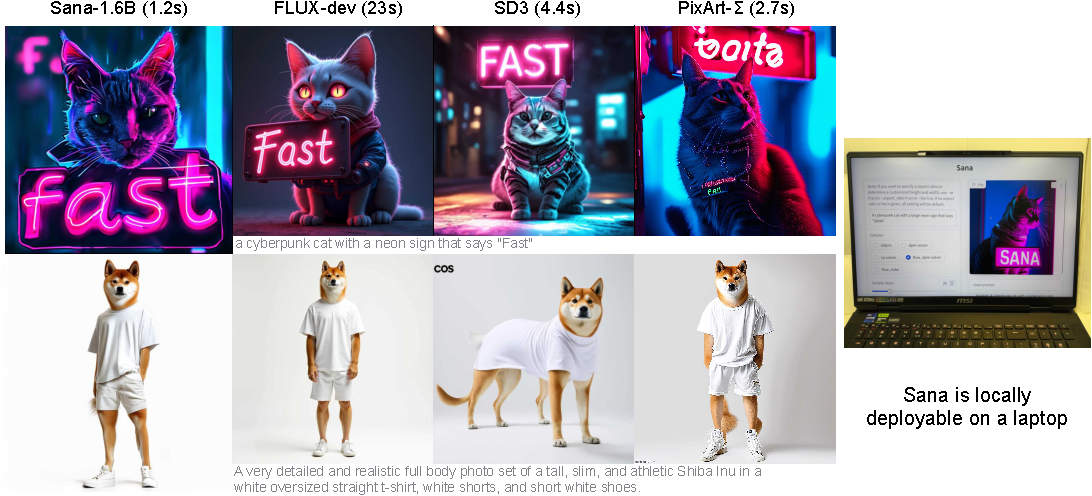
\includegraphics[width=0.99\textwidth]{figures/vis_compare.pdf}
    \caption{\textbf{Left}: Visualization comparison of \model{}-1.6B vs FLUX-dev, SD3 and PixArt-$\Sigma$. The speed is tested on an A100 GPU with FP16 precision.
    \textbf{Right}: Quantize \model{}-1.6B is deployable on a GPU laptop generating an 1K$\times$1K image within 1 seconds.}
    \label{fig:vis_compare}
    \vspace{-0.5em}
\end{figure}
